\documentclass{beamer}
%\usetheme{Boadilla}
\usepackage[latin1]{inputenc}
\usepackage{ upgreek }
\usepackage{verbatim} 

\usepackage{amssymb}
\usepackage{graphicx}
\usepackage{url}
\usepackage{verbatim} 

\usetheme{Warsaw}
\title{Semantic Labeling of 3D Point Clouds for indoor scenes}


\begin{document}
\begin{frame}
\titlepage
\end{frame}

\begin{frame}{Motivation}
	\begin{figure}[t!]
		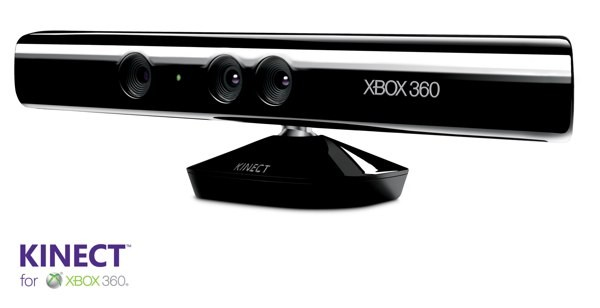
\includegraphics[width=.5\linewidth]{kinect.jpg}
	\end{figure}

	\begin{itemize}
		\item 3D era for robots has arrived 
		\item  cheap, fast 3D machine vision
		\item  both color and depth available
	\end{itemize}

\end{frame}

\begin{frame}{Introduction}
	\begin{itemize}
		\item How does a kinect pointcloud look like? \footnote{http://arstechnica.com/gaming/news/2010/11/bathed-in-light-how-the-kinect-paints-your-room-in-ir-video.ars}

	\end{itemize}
\end{frame}

\begin{frame}{Introduction}
	\begin{itemize}
		\item Desired goal: labeled pointcloud:(show)

	\end{itemize}
\end{frame}

\begin{frame}{Approach}
	\begin{itemize}
		\item stitching:(show)
		\item  segmentation:(show)
		\item  graph construction(show using graphviz?)
		\item  feature generation
		\item  inference
	\end{itemize}

\end{frame}

\begin{frame}{Captured Properties}
	\begin{itemize}
		\item Visual Appearance
		\item  Local Shape and Geometry
		\item  Geometrical Context
	\end{itemize}

\end{frame}

\begin{frame}{Visual Appearance}
match the following to table/printer
\begin{figure}[t!]

\includegraphics[width=.3\linewidth]{printer-small.png}
\hskip .2in

\includegraphics[width=.3\linewidth]{table-small.png}
\end{figure}
\end{frame}

\begin{frame}{Visual Appearance}

\begin{figure}[t!]
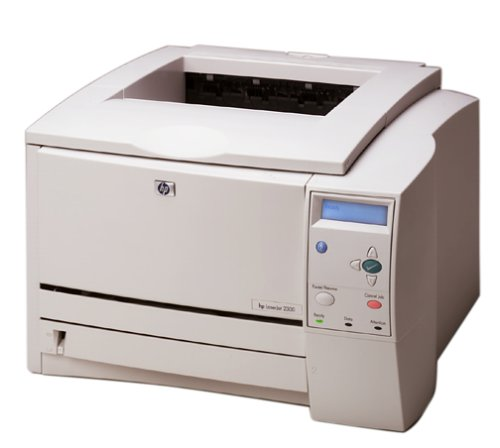
\includegraphics[width=.4\linewidth]{printer.jpg}
\hskip .2in
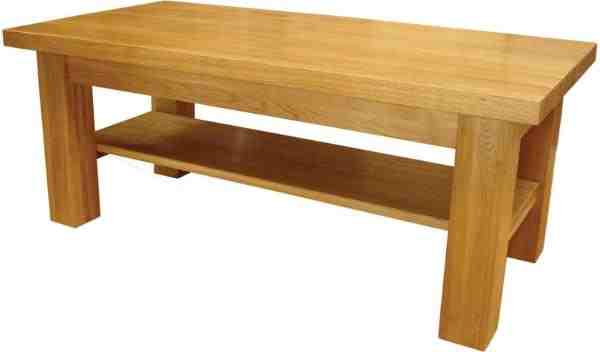
\includegraphics[width=.4\linewidth]{table.jpg}
\end{figure}
\end{frame}

\begin{frame}{Visual Appearance}

\begin{figure}[t!]
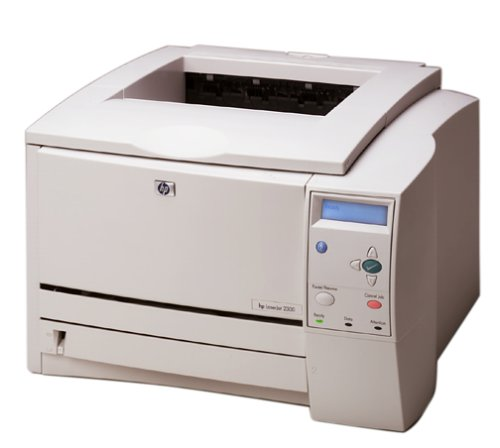
\includegraphics[width=.4\linewidth]{printer.jpg}
\hskip .2in
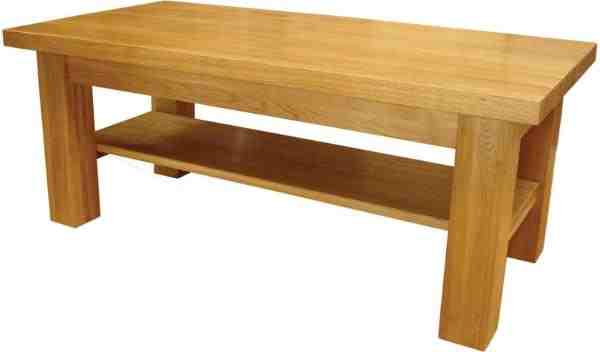
\includegraphics[width=.4\linewidth]{table.jpg}
\end{figure}
\end{frame}

\begin{frame}{Geometrical Context}
pic: monitor near CPU blurred out
\end{frame}

\begin{frame}{Model}

\end{frame}

\begin{frame}{Features}

\end{frame}

\begin{frame}{Learning}

\end{frame}

\begin{frame}{Inference}
 
 
\end{frame}

\begin{frame}{Data}
% types and number of scene 
% examples of labeled pointclouds

\end{frame}


\begin{frame}{Results }
% put table
% put confusion matrices 
% discuss the points mentioned in the paper  
\end{frame}

\begin{frame}{Robotic Experiments}
% setup
%demo
% table of results
\end{frame}

\begin{frame}{Current Work: }
\end{frame}

\begin{frame}{Current Work: }
\end{frame}

\end{document} 
